\documentclass[twoside,10pt,a4paper]{article}

%================================ PREAMBLE ==================================

%--------- Packages -----------
\usepackage{fullpage}
\usepackage{amssymb}
\usepackage{amsmath}
\usepackage{amsthm}
\usepackage{latexsym}
\usepackage{graphicx}
\usepackage{tikz}				% sophisticated graphics package
\usepackage{color}
\usepackage{hyperref}
%\usepackage{algorithm,algorithmic}

%----------Spacing-------------
\setlength{\oddsidemargin}{0.25 in}
\setlength{\evensidemargin}{-0.25 in}
\setlength{\topmargin}{-0.6 in}
\setlength{\textwidth}{6.5 in}
\setlength{\textheight}{9.4 in}
\setlength{\headsep}{0.75 in}
\setlength{\parindent}{0 in}
\setlength{\parskip}{0.1 in}

%----------Header--------------
\newcommand{\assignmentreport}[4]{
   \pagestyle{myheadings}
   \thispagestyle{plain}
   \newpage
   \setcounter{page}{1}
   \noindent
   \begin{center}
   \framebox{
      \vbox{\vspace{2mm}
    \hbox to 6.28in { {\bf E0 270 Machine Learning} \hfill {\it Due:} #2 }
       \vspace{6mm}
       \hbox to 6.28in { \hfill {\Large Assignment #1 - Report} \hfill }
       \vspace{6mm}
       \hbox to 6.28in {{\it #3} \hfill {\it #4} }
      \vspace{2mm}}
   }
   \end{center}
   \markboth{Assignment #2 :\it #3,\it#4}{Assignment #2: \it #3,\it#4}
   \vspace*{4mm}
}

%--------Environments----------
\theoremstyle{definition}
\newtheorem{thm}{Theorem}[section]
\newtheorem{lem}[thm]{Lemma}
\newtheorem{prop}[thm]{Proposition}
\newtheorem{cor}[thm]{Corollary}
\newenvironment{pf}{{\noindent\sc Proof. }}{\qed}
\newenvironment{map}{\[\begin{array}{cccc}} {\end{array}\]}

\theoremstyle{definition}
\newtheorem*{defn}{Definition}
\newtheorem{exmp}{Example}
\newtheorem*{prob}{Problem}
\newtheorem*{exer}{Exercise}

\theoremstyle{remark}
\newtheorem*{rem}{Remark}
\newtheorem*{note}{Note}

%---------Definitions----------
\newcommand{\Fig}[1]{Figure~\ref{#1}}
\newcommand{\Sec}[1]{Section~\ref{#1}}
\newcommand{\Tab}[1]{Table~\ref{#1}}
\newcommand{\Tabs}[2]{Tables~\ref{#1}--\ref{#2}}
\newcommand{\Eqn}[1]{Eq.~(\ref{#1})}
\newcommand{\Eqs}[2]{Eqs.~(\ref{#1}-\ref{#2})}
\newcommand{\Lem}[1]{Lemma~\ref{#1}}
\newcommand{\Thm}[1]{Theorem~\ref{#1}}
\newcommand{\Cor}[1]{Corollary~\ref{#1}}
\newcommand{\App}[1]{Appendix~\ref{#1}}
\newcommand{\Def}[1]{Definition~\ref{#1}}
%
\renewcommand{\>}{{\rightarrow}}
\newcommand{\R}{{\mathbb R}}
\newcommand{\Z}{{\mathbb Z}}
\newcommand{\N}{{\mathbb N}}
\renewcommand{\P}{{\mathbf P}}
\newcommand{\E}{{\mathbf E}}
\newcommand{\Var}{{\mathbf{Var}}}
\newcommand{\I}{{\mathbf I}}
\newcommand{\1}{{\mathbf 1}}
\newcommand{\0}{{\mathbf 0}}
\renewcommand{\H}{{\mathcal H}}
\newcommand{\F}{{\mathcal F}}
\newcommand{\G}{{\mathcal G}}
\renewcommand{\L}{{\mathcal L}}
\newcommand{\cN}{{\mathcal N}}
\newcommand{\X}{{\mathcal X}}
\newcommand{\Y}{{\mathcal Y}}
\newcommand{\sign}{\textup{\textrm{sign}}}
\newcommand{\er}{\textup{\textrm{er}}}
\newcommand{\abs}{\textup{\textrm{abs}}}
\newcommand{\sq}{\textup{\textrm{sq}}}
\newcommand{\zo}{\textup{\textrm{0-1}}}
\newcommand{\hinge}{\textup{\textrm{hinge}}}
\newcommand{\ramp}{\textup{\textrm{ramp}}}
\newcommand{\mar}{\textup{\textrm{margin}}}
\newcommand{\lin}{\textup{\textrm{lin}}}
\newcommand{\poly}{\textup{\textrm{poly}}}
\newcommand{\majority}{\textup{\textrm{majority}}}
\newcommand{\maj}{\textup{\textrm{maj}}}
\newcommand{\co}{\textup{\textrm{co}}}
\newcommand{\agg}{\textup{\textrm{agg}}}
\newcommand{\bad}{\textup{\textrm{bad}}}
\newcommand{\EX}{\textup{\textrm{\textit{EX}}}}
\newcommand{\GD}{\textup{\textrm{{GD}}}}
\newcommand{\EG}{\textup{\textrm{{EG}}}}
\newcommand{\algorithm}{\textup{\textrm{{algorithm}}}}
\newcommand{\VCdim}{\textup{\textrm{{VCdim}}}}
\newcommand{\VCentropy}{\textup{\textrm{{VC-entropy}}}}
\newcommand{\Pdim}{\textup{\textrm{{Pdim}}}}
\newcommand{\fat}{\textup{\textrm{{fat}}}}
\newcommand{\x}{{\mathbf x}}
\newcommand{\w}{{\mathbf w}}
\newcommand{\p}{{\mathbf p}}
\newcommand{\q}{{\mathbf q}}
\renewcommand{\r}{{\mathbf r}}
\renewcommand{\u}{{\mathbf u}}
\renewcommand{\b}{{\mathbf b}}
\newcommand{\bloss}{{\boldsymbol \ell}}
\newcommand{\balpha}{{\boldsymbol \alpha}}
\newcommand{\bxi}{{\boldsymbol \xi}}
\newcommand{\bpsi}{{\boldsymbol \psi}}
\newcommand{\btau}{{\boldsymbol \tau}}

% colors
\definecolor{mygreen}{RGB}{44,85,17}				% for emphasizing text (#2c5511)
\definecolor{myblue}{RGB}{34,31,217}					% for emphasizing text (#5d90c2)
\definecolor{mybrown}{RGB}{194,164,113}			% for emphasizing text (#c2a471)
\definecolor{myred}{RGB}{255,66,56}					% for emphasizing text (#cc7b76)
\newcommand*{\mygreen}[1]{\textcolor{mygreen}{#1}}
\newcommand*{\myblue}[1]{\textcolor{myblue}{#1}}
\newcommand*{\mybrown}[1]{\textcolor{mybrown}{#1}}
\newcommand*{\myred}[1]{\textcolor{myred}{#1}}

% box 
\newcommand*{\mybox}[2]{% width, content
	\par\noindent
	\begin{tikzpicture}[
		mynodestyle/.style={rectangle,draw=mygreen,
											 thick,inner sep=2mm,text justified,top color=white,
											 bottom color=white,above}]%
		\node[mynodestyle,at={(0.5*#1+2mm+0.4pt,0)}]{%
			\begin{minipage}[t]{#1}
				#2
			\end{minipage}%
		};
	\end{tikzpicture}%	
	\par\vspace{-1.3em}
}


%=============================== END PREAMBLE ===============================

%============================ BEGIN DOCUMENT ================================

\begin{document}

%Use the following format: \assignmentreport{Assignment number}{Due date}{Your name}{SR Number}

\assignmentreport{6}{Apr 17, 2012}{Sachin Nagargoje}{04-04-00-10-41-11-1-08449}

%-----------------------

\section{Solution: Problem 1}
Consider the unit circle in the figure below.\\

\begin{center}
\scalebox{1.25}{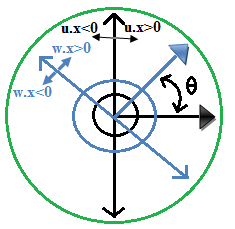
\includegraphics{./ml62}}
\end{center}
The black line represents unit vector $u$ and the green line represents unit vector $w$.
The angle between them is $\theta$. 
As we can see from figure, each of these vectors partitions the whole space $\mathbb{R}^2$ into two subspaces.
One of these subspaces contains the vectors for which the dot-product is positive and the other subspace contains the vectors for which the dot-product is negative.
Thus, given two vectors $u$ and $w$, partitions S into 4 subspaces containing the vectors x,such that \\
\begin{enumerate}
 \item $u.x \ge 0$ and $w.x \ge 0$ subtending angle $\pi - \theta $ at the center of unit circle.
 \item $u.x \le 0$ and $w.x \ge 0$ subtending angle $\theta $ at the center of unit circle.
 \item $u.x \ge 0$ and $w.x \le 0$ subtending angle $\theta $ at the center of unit circle.
 \item $u.x \le 0$ and $w.x \le 0$ subtending angle $\pi - \theta $ at the center of unit circle.
\end{enumerate}
where the equality holds only at the corresponding lines and $\theta$ is given by, \\
\begin{center}
$cos(\theta) = \frac{u.w}{{\|u\|}_2 {\|w\|}_2} = u.w$ 
\end{center}
since ${\|u\|}_2 = {\|w\|}_2 = 1 $. \\
Thus the probability that $w.x$ and $u.x$ will have different signs , i.e. \\
\begin{center}
\mybox{0.5\textwidth}{ $\mathbb{P}_{x \in S}[sign(w.x) \ne sign(u.x) ] = \frac{2\theta}{2\pi} = \frac{\theta}{\pi}= \frac{cos^{-1}(u.w)}{\pi} $ }
\end{center}



\section{Solution: Problem 2}
\subsection{Part a}

Ratio of the number of mistakes made relative to the total number of examples
seen as a function of the number of examples seen \\

 \begin{center}
 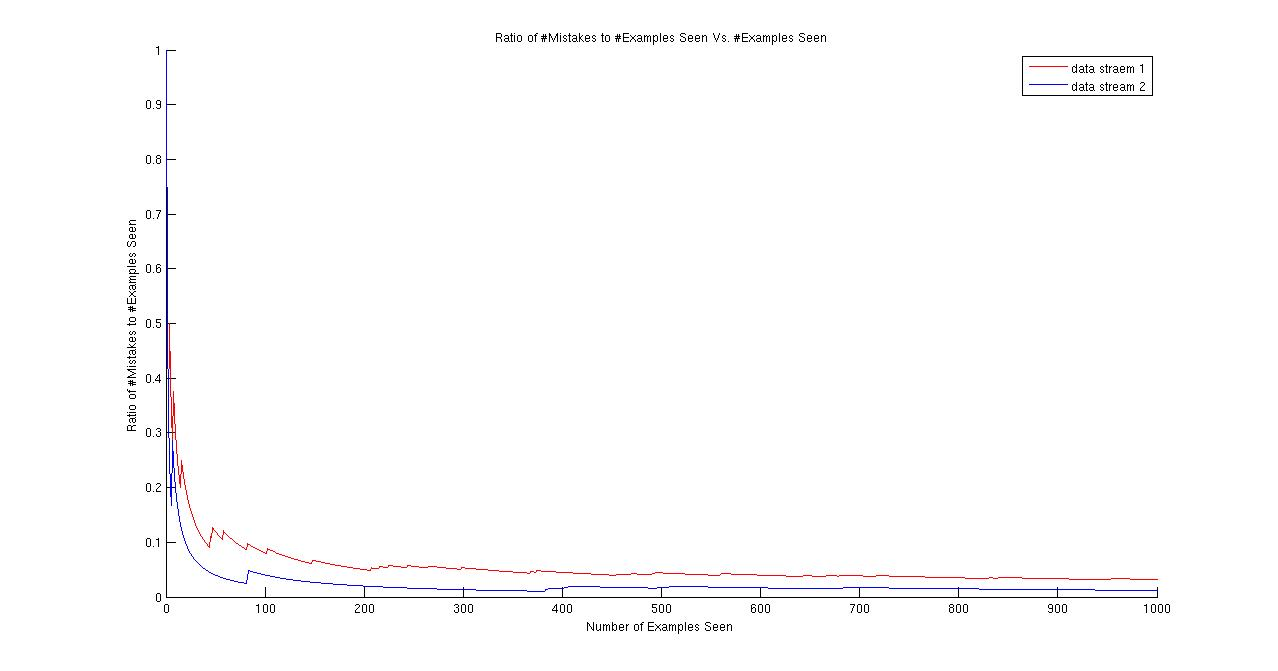
\includegraphics[scale=0.4]{./finale/2a1} 
 % RatioVsEg.jpg: 1278x447 pixel, 72dpi, 45.08x15.77 cm, bb=0 0 1278 447
\end{center}
\newpage
Upper bound on this ratio obtained from the mistake bound for data stream 1 \\

 \begin{center}
 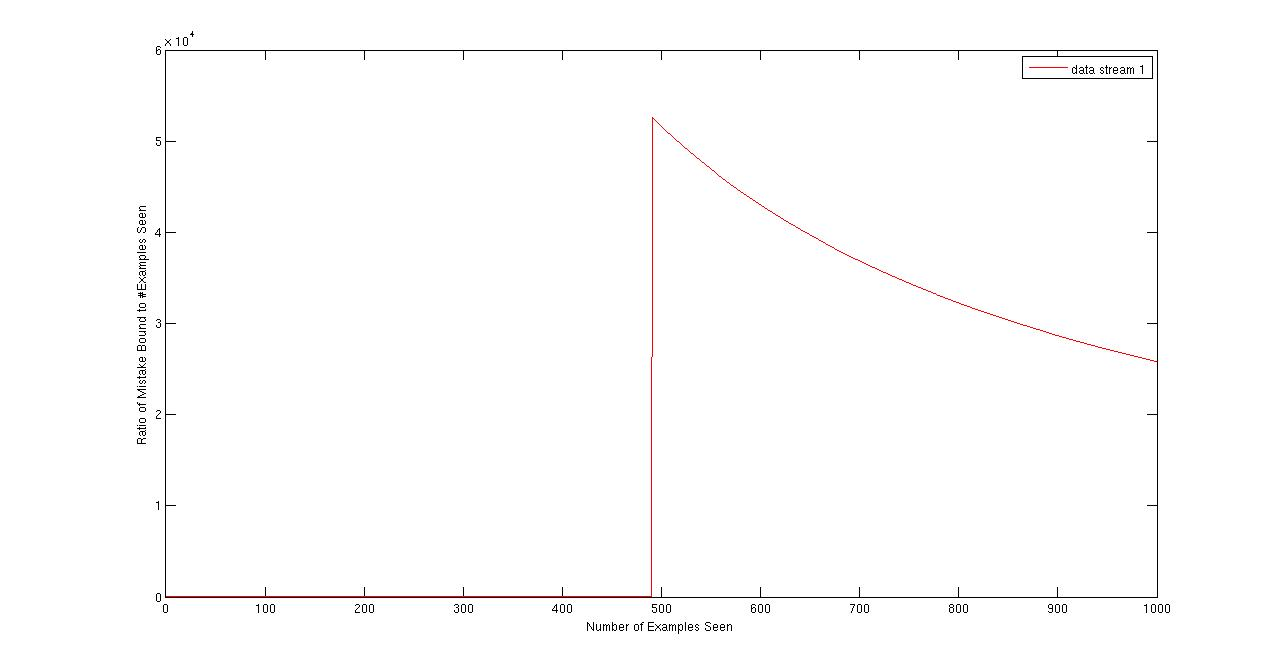
\includegraphics[scale=0.4]{./finale/2a2}
 % RatioVsEg.jpg: 1278x447 pixel, 72dpi, 45.08x15.77 cm, bb=0 0 1278 447
\end{center}


Upper bound on this ratio obtained from the mistake bound for data stream 2 \\

 \begin{center}
 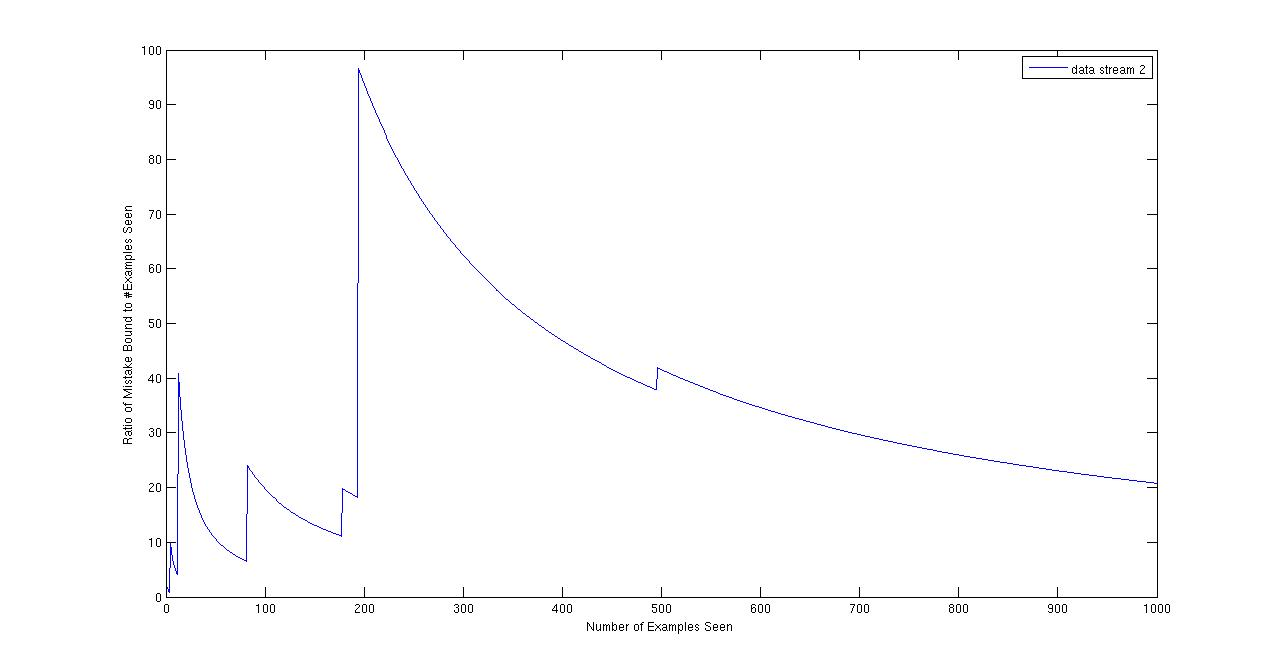
\includegraphics[scale=0.4]{./finale/2a3}
 % RatioVsEg.jpg: 1278x447 pixel, 72dpi, 45.08x15.77 cm, bb=0 0 1278 447
\end{center}

Upper bounds for data stream 1 and 2, comparison on log scale. \\

 \begin{center}
 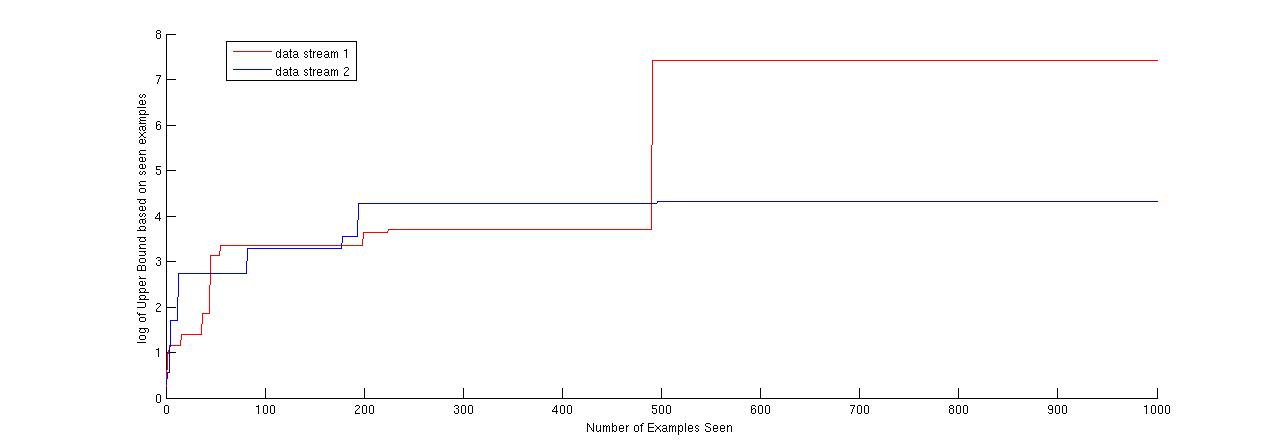
\includegraphics[scale=0.4]{./ub2log.jpg}
 % RatioVsEg.jpg: 1278x447 pixel, 72dpi, 45.08x15.77 cm, bb=0 0 1278 447
\end{center}

\subsection{Part b}
Expected error of the linear predictor learned by the perceptron algorithm as a function of the number of examples seen. \\

\begin{center}
 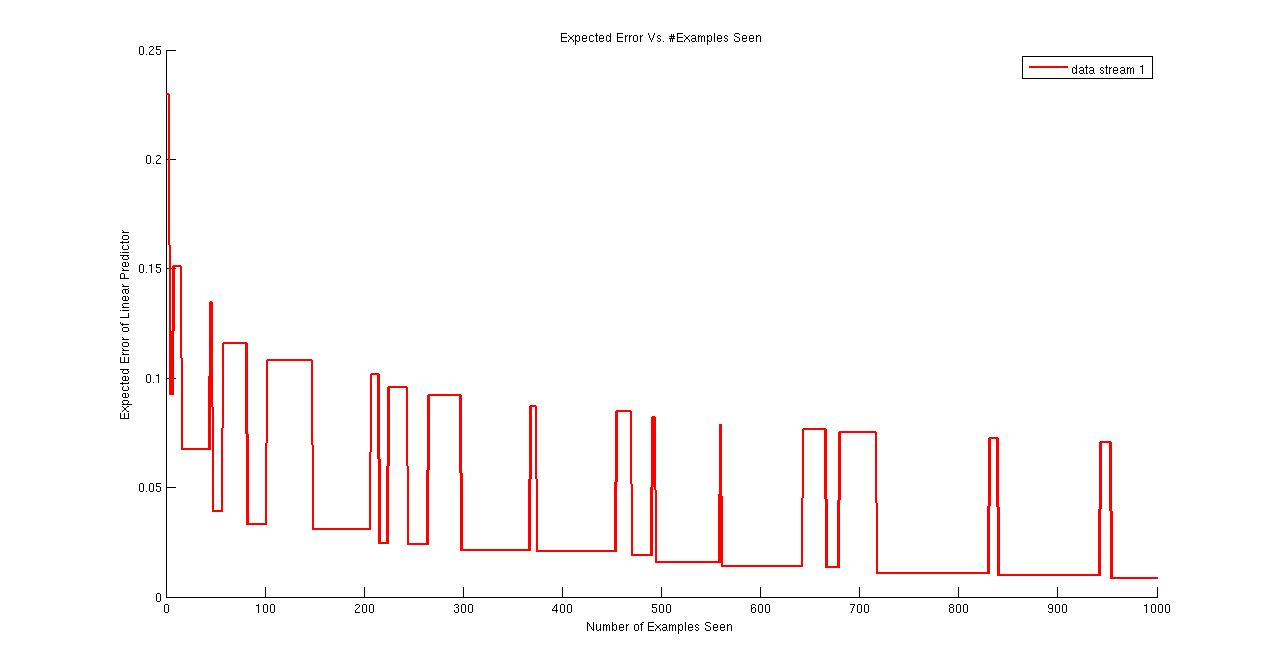
\includegraphics[scale=0.37,keepaspectratio=true]{./finale/2b1}
 % ExErrVsEg.jpg: 1278x447 pixel, 72dpi, 45.08x15.77 cm, bb=0 0 1278 447
\end{center}
 
\newpage

\section{Solution: Problem 3}
Number of labels requested as a function of the number of examples seen\\
\begin{center}
 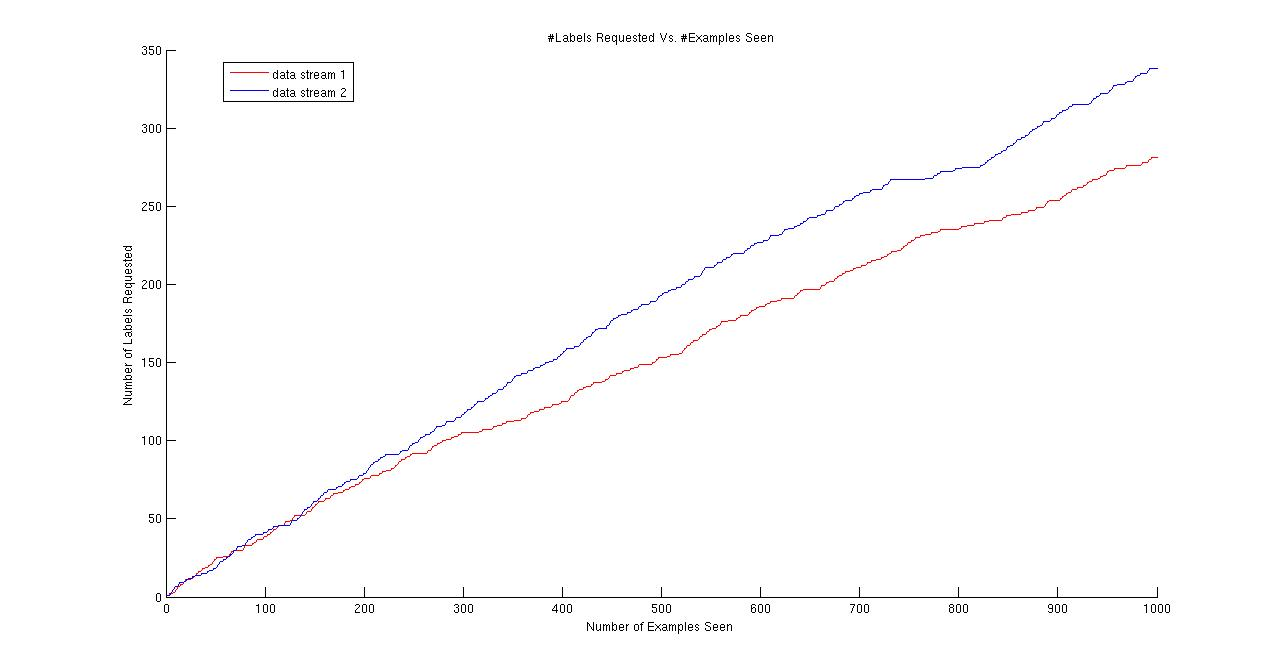
\includegraphics[scale=0.35]{./finale/3a1.jpg}
 % 3a1.jpg: 1278x671 pixel, 72dpi, 45.08x23.67 cm, bb=0 0 1278 671
\end{center}

Ratio of the number of mistakes made relative to the total number of examples seen as a function of the number of examples seen\\
\begin{center}
 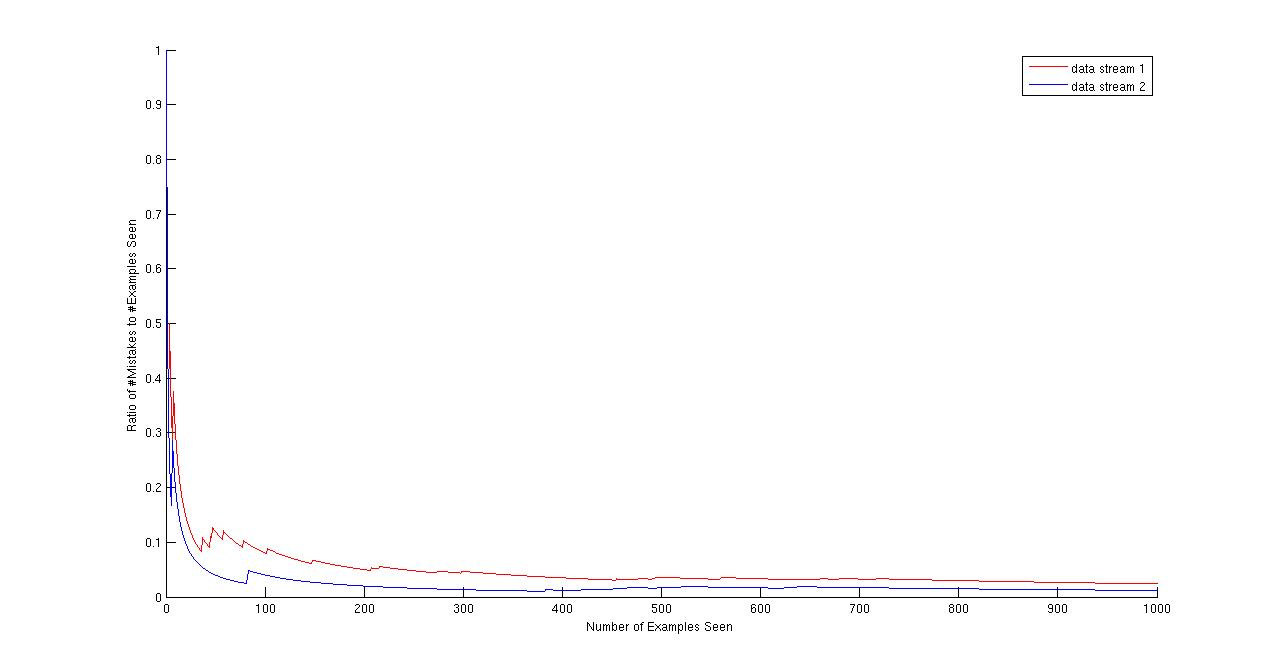
\includegraphics[scale=0.35]{./finale/3a2.jpg}
 % 3a2.jpg: 1278x671 pixel, 72dpi, 45.08x23.67 cm, bb=0 0 1278 671
\end{center}
Comparing this plot with plot in 2(a), we get that the final value is lower in this case.

\newpage

Expected error as a function of the number of labels requested\\
\begin{center}
 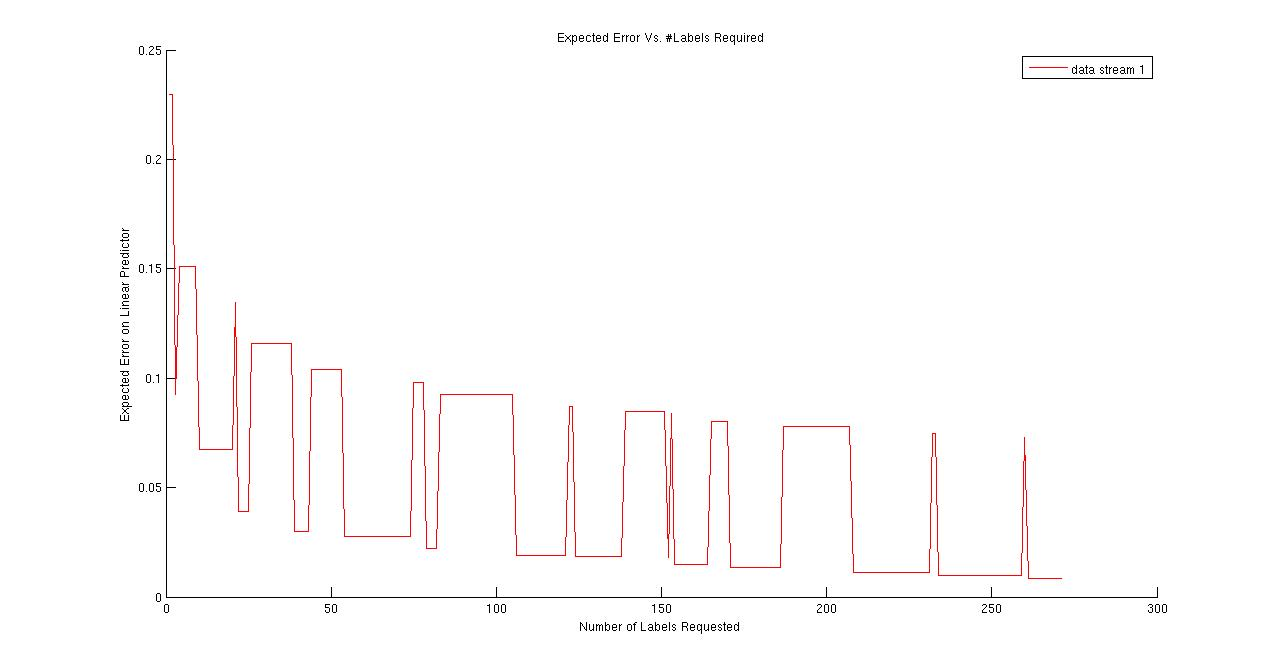
\includegraphics[scale=0.35]{./finale/3b1.jpg}
 % 3b1.jpg: 1278x671 pixel, 72dpi, 45.08x23.67 cm, bb=0 0 1278 671
\end{center}


\section{Solution: Problem 4}
The solution to problem 1 holds good here for $n-dimensioal$ space as well.\\
Let $U$ and $W$ be the two hyperplanes, defined by the vectors $u$ and $w$ respectively i.e. planes containing all the vectors which are \textit{orthogonal} to vectors $u$ and $w$ respectively.
These two hyperplanes will partition $S$ into four parts containing vectors $x$ (similar to the solution 1) such that, \\ 
\begin{enumerate}
 \item $u.x \ge 0$ and $w.x \ge 0$ .
 \item $u.x \le 0$ and $w.x \ge 0$ .
 \item $u.x \ge 0$ and $w.x \le 0$ .
 \item $u.x \le 0$ and $w.x \le 0$ .
\end{enumerate}

Let $\theta$ be the angle between the vectors $u$ and $w$ in the $2-dimensioal$ plane containing vectors $u$ and $w$. 
The intersection of the $2-dimensional$ plane containing $u$ and $w$ with the unit sphere will be a circle. Now the projections of all the vectors in $S$ on the plane containing $u$ and $w$ will form concentric circles and exactly $2^{(n-2)}$ vectors in $S$ will have same projections.\\
Thus, distribution of vectors in S is still uniform and this problem reduces to a problem similar to problem-1. \\
Thus the probability that $w.x$ and $u.x$ will have different signs , i.e. \\
\begin{center}
\mybox{0.5\textwidth}{ $\mathbb{P}_{x \in S}[sign(w.x) \ne sign(u.x) ] = \frac{2\theta}{2\pi} = \frac{\theta}{\pi}= \frac{cos^{-1}(u.w)}{\pi} $ }
\end{center}

\end{document}

%=========================== END DOCUMENT ==============================

